\chapter{Methodology}

In this section we introduce our proposed method for SDP, Figure 3.1 is the overview of our method. we separate our method into 6 part. 

\begin{figure}
    \centering
    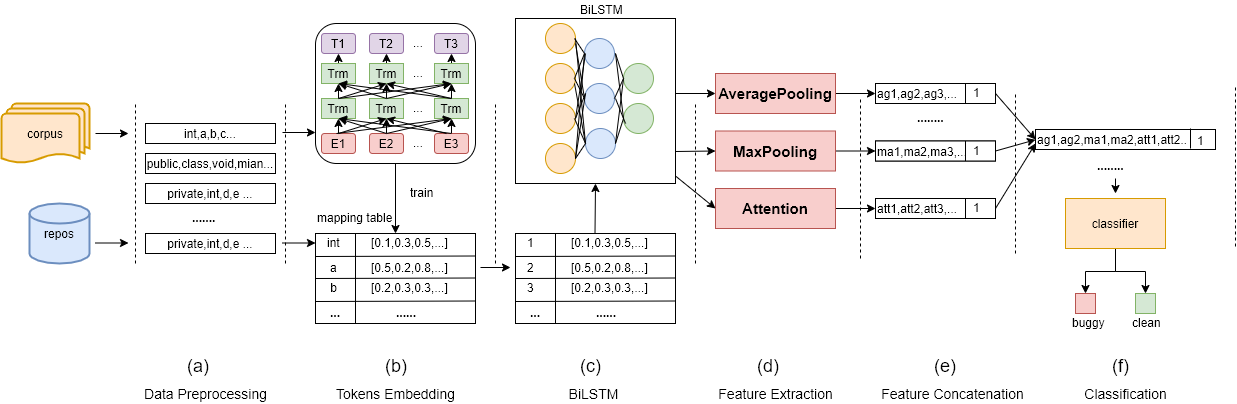
\includegraphics[width=\textwidth,height=0.2\textheight]{pic/model_overview.png}
    \caption{model overview}
    \label{fig:my_label}
\end{figure}

% proprocessing for both dataset and corpus
\section{Data Preprocessing}
In this section, we preprocess our dataset and corpus that fit training, we need to process data and corpus to fit our model. To extract the semantics feature of a program, many research use ASTs (Abstract Synatx Trees) \cite{}to present the semantics of files. However, they just select some forms of nodes from ASTs then concatenate with them, which destroyed the order if original program. Besides, since context information not only hidden in single token, but decided by sequence of tokens. Based on these problem, we directly tokenize Java files. The step can be describled as follow:
%这个地方说明有待加强
\begin{itemize}
    \item Comment removal.We remove all blank lines and comments.
    \item Sequence generation. we directly tokenize all the data to generate the sequence. for each files
    \item We filter out all punctuation and \textbf{string} since we believe it contain less information.
    \item Vocabulary building. We merge all sequence in a project, then count each token's frequency, finally rank each token according to its frequency. We also replace those token whose frequency are lower than our setting with "\textit{unk}". Finally, we padding each sequence wit fixed length.
\end{itemize}

during the processing, we remove all the tokens that has useless information. such as the \texttt{import},\texttt{package} tokens.
% 这个地方图片补充(四张不同的情景图)
% need to explain why 
\subsection{Data Augmentation}
In our dataset, the amount of instance of most projects is no more than 1,000, previous research many focus on data imbalance. However, the entire dataset are still not enough. On the other hand, deep learning method need large volume dataset to train effective model, otherwise, it would be overfitting and is not convincing. Thereby, to construct well-trained data, we learn from method proposed by Li \cite{} to generate specific volume data we need. we generate sequences from one sequence by using following four strategies:
\begin{itemize}
    \item \textbf{Similiar Tokens Replace}. We randomly replace similar tokens for software defect prediction with large corpus 
    \item \textbf{Randomly Insert}. We randomly insert several kinds of tokens into original sequence.
    \item \textbf{Randomly Swap}. We randomly swap two tokens in a sequence.
    \item \textbf{Randomly Delete}. We randomly delete tokens in sequence. 
\end{itemize}

% 这个地方待补充(图和说明)
\section{Token Embedding}
In deep learning process, word embedding is necessary stage for downstream task such as text classification, question answering and machine translation. It is also necessary to make token embedding for our model to yeild the suitable data for training. Thereby, we need to embedding our data to generate model. \\
\textbf{TODO}

\section{Feature Extraction}
\textbf{TODO}
\section{Feature Concatenation}
\textbf{TODO}
\section{Classification}
\textbf{TODO}